\begin{center}
    {\huge Chapter 1}
\end{center}
\section*{Problem 5}
No, we can prove by deriving a recurrence relation for the number of regions created by $n$ circles.

Let, $C_n$ be the number of regions created by $n$ circles. Then,
\begin{itemize}
    \item For $C_0$, we have no circle, only a single region. Therefore, $C_0 = 1$.
    \item For $C_1$, we have an inner and an outer region. So $C_1 = 2$.
    \item Suppose we add the $n$th circle, and it intersects the previous $(n-1)$ circles. For each circle the new one intersects with, it creates 2 additional regions.
          \begin{figure}[h!]
              \centering
              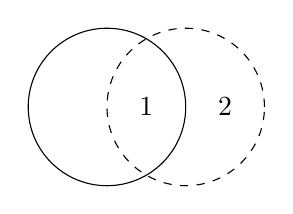
\begin{tikzpicture}
                  \draw (0,0) circle (1cm);
                  \draw[dashed] (1,0) circle (1cm);
                  \node at (0.5,0) {1};
                  \node at (1.5,0) {2};
              \end{tikzpicture}
          \end{figure}

          So, for $n \geq 2$,
          \begin{align*}
              C_n & = C_{n-1} + 2\times(n-1)                                             \\
                  & = C_{n-2} + 2\times(n-2) + 2\times(n-1)                              \\
                  & = C_{1} + 2\times1 + 2\times2 + \ldots + 2\times(n-2) + 2\times(n-1) \\
                  & = 2 + 2\times(1+2+\ldots+(n-2)+(n-1))                                \\
                  & = 2+2\times\frac{n(n-1)}{2}                                          \\
                  & = n^2-n+2                                                            \\
          \end{align*}
          For $n=4$, we get $C_4=14$. We can have at most $14$ regions ($13$ inner, $1$ outer) with $4$ circles intersecting each other.
          \begin{figure}[h!]
              \centering
              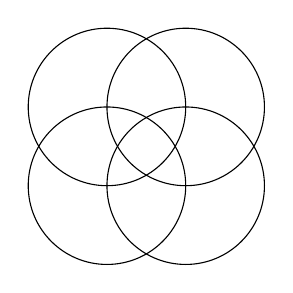
\begin{tikzpicture}
                  \draw (0,0) circle (1cm);
                  \draw (1,0) circle (1cm);
                  \draw (0,1) circle (1cm);
                  \draw (1,1) circle (1cm);
              \end{tikzpicture}
          \end{figure}
\end{itemize}
\clearpage
\section*{Problem 6}
In the original problem, the maximum number of regions, both bounded and unbounded for $n$ line segments was bounded by $O(n^2)$. So, the maximum number of \textit{only bounded} regions must also be bounded by $O(n^2)$.

Let us assume that the solution is $B_n=an^2+bn+c$, where $B_n$ indicates the maximum number of bounded regions possible by $n$ straight lines.
\begin{itemize}
    \item For $n=1$, we have a single line, and no bounded regions, hence $B_1 = 0$.
          \begin{equation}
              a+b+c=0 \tag{1}
          \end{equation}
    \item For $n=2$, we have two intersecting lines, and no bounded regions. Hence $B_2=0$.
          \begin{equation}
              4a+2b+c=0 \tag{2}
          \end{equation}
          \vspace{-.5cm}
          \begin{figure}[h!]
              \centering
              \begin{tikzpicture}
                  \draw (0,0) -- (2,2);
                  \draw (1.3,0) -- (1.3,2);
              \end{tikzpicture}
          \end{figure}
    \item For $n=3$, we have a single bounded region, so $B_3=1$.
          \begin{equation}
              9a+3b+c = 1 \tag{3}
          \end{equation}
          \vspace{-.5cm}
          \begin{figure}[h!]
              \centering
              \begin{tikzpicture}
                  \draw (0,0) -- (2,2);
                  \draw (1.4,0) -- (1.4,2);
                  \draw (0,0.3) -- (2, 0.3);
              \end{tikzpicture}
          \end{figure}
\end{itemize}
Solving these system of equations $(1), (2) \text{ and } (3)$, we get:
\begin{align*}
    a   & =\frac{1}{2}                        \\
    b   & =-\frac{3}{2}                       \\
    c   & =1                                  \\
    B_n & =\frac{n^2}{2} - \frac{3n^2}{2} + 1
\end{align*}
\clearpage

\section*{Problem 10}
We denote the other peg as $C$. For this problem, we can move the disks only clockwise, that is either from $A$ to $B$, $B$ to $C$ or $C$ to $A$. From the problem statement,
\begin{enumerate}[label=(\roman*)]
    \item $Q_n$ is the number of moves required to shift $n$ disks from peg $A$ to peg $B$ under the given restrictions. Since the moves are symmetric, shifting $n$ disks from $B$ to $C$ or $C$ to $A$ require the same number of moves as shifting from $A$ to $B$.
    \item $R_n$ is the number of moves required to shift $n$ disks from $B$ to $A$. By the same reasoning, shifting $n$ disks from $C$ to $B$ or $A$ to $C$ also require $R_n$ number of moves.
\end{enumerate}

\tikzfig{fig10_1} $\implies Q_n =$

\tikzfig{fig10_2} $ R_{n-1}$ (move $n-1$ disks from $A$ to $C$)\\

\tikzfig{fig10_3} $ +1$ (move $n$th disk from $A$ to $B$)\\

\tikzfig{fig10_4} $ +R_{n-1}$ (move $n-1$ disks from $C$ to $B$)

\begin{align}
    Q_n & = R_{n-1} + 1 + R_{n-1} \nonumber \\
        & =2R_{n-1} + 1 \label{eq:10_1}
\end{align}

\tikzfig{fig10_10} $\implies R_n=$\\
\tikzfig{fig10_5} $R_{n-1}$ (move $n-1$ disks from $B$ to $A$)\\
\tikzfig{fig10_6} $+1$ (move $n$th disk from $B$ to $C$)\\
\tikzfig{fig10_7} $+Q_{n-1}$ (move $n-1$ disks from $A$ to $B$)\\
\tikzfig{fig10_8} $+1$ (move $nth$ disk from $C$ to $A$)\\
\tikzfig{fig10_9} $+R_{n-1}$ (move $n-1$ disks from $B$ to $A$)
\begin{align}
    R_n & = R_{n-1} + 1 + Q_{n-1} + 1 + R_{n-1} \nonumber \\
        & =2R_{n-1} + 2 + Q_{n-1} \label{eq:10_2}
\end{align}

From \eqref{eq:10_1}, we can rewrite $2R_{n-1}$ as:
\begin{align}
    2R_{n-1} = Q_n - 1
\end{align}

Replacing this in \eqref{eq:10_2}, we get:
\begin{align}
    R_n & = Q_n - 1 + 2 + Q_{n-1} \nonumber \\
        & = Q_n + Q_{n-1} + 1
\end{align}
Therefore,

\begin{minipage}{.5\textwidth}
    \begin{equation*}
        Q_n =
        \begin{cases}
            0            & \text{if } n=0   \\
            2R_{n-1} + 1 & \text{if } n > 0
        \end{cases}
    \end{equation*}
\end{minipage}%
\begin{minipage}{0.5\textwidth}
    \begin{equation*}
        R_n =
        \begin{cases}
            0                 & \text{if } n=0   \\
            Q_n + Q_{n-1} + 1 & \text{if } n > 0
        \end{cases}
    \end{equation*}
\end{minipage}
\section*{Problem 11}
\begin{enumerate}
    \item Since each of the disks contains an identical copy, we would need exactly 2 moves for moving a single disk including its copy form one peg to another. Hence the total number of moves is just the twice of the original solution, that is $2 \times (2^n-1)$.
          \begin{figure}[h!]
              \centering
              \tikzfig{fig11_1}
              \caption*{Each disk of the same size is indistinguishable from its pair}
              \label{fig:fig11_1}
          \end{figure}
    \item Now the disks contain a copy of the same size, but each of the copies is now \textit{distinguishable} from its pair. The additional constraint now imposed is that we would like to shift the disks in a way so that the original ordering is maintained.
          \begin{figure}[h!]
              \centering
              \tikzfig{fig11_2}
              \label{fig:fig11_2}
          \end{figure}

          We distinguish each pair by giving alternating colors. We can interpret the given constraint in this way:

          ``\textit{The final arrangement should not contain any black disk under a white disk of the same size.}''
\end{enumerate}

This rephrased constraint ensures that the original ordering in the initial arrangement is maintained in the final arrangement. Let us assume that we need $D_{n}$ moves to move such a stack of disks under the given constraints from one peg to another.
\clearpage

\tikzfig{fig11_3} $\implies D_n = $\\
\tikzfig{fig11_4} $D_{n-1} +$\\
\tikzfig{fig11_5} $1 +$\\
\tikzfig{fig11_6} $D_{n-1}+$ \\
\tikzfig{fig11_7} $1+$\\
\tikzfig{fig11_8} $D_{n-1}+$\\
\tikzfig{fig11_9} $1+$\\
\tikzfig{fig11_10} $D_{n-1}$

\begin{align}
    D_n & = D_{n-1} + 1 + D_{n-1} + 1 + D_{n-1} + 1 + D_{n-1} \nonumber \\
        & = 4D_{n-1} + 3
\end{align}

In order to solve this recurrence, we can simplify a bit. We first add $1$ to both sides, giving:
\begin{align*}
    D_n + 1 & = 4D_{n-1} + 4  \\
            & =4(D_{n-1} + 1)
\end{align*}
If we let $Z_n = D_n + 1$, we get:
\begin{align*}
    Z_n & = 4Z_{n-1}
\end{align*}
Since $D_0=0$, $Z_0 = D_0 + 1 = 1$, we can simply unwind the recurrence and find the solution to $Z_n$ directly:
\begin{align*}
    Z_n          & = 4^n   \\
    \implies D_n & = 4^n-1
\end{align*}
\clearpage

\section*{Problem 13}
Let $ZZ_n$ denote the maximum number of regions defined by $n$ zig-zag lines. Here,
\begin{align*}
    ZZ_0 & = 1 \\
    ZZ_1 & = 2
\end{align*}
To find a recurrence relation, we notice the following:
\begin{enumerate}[label=(\roman*)]
    \item Assume we are dealing with straight lines only, no zig-zags. When the $n$th line intersects the previous $n-1$ lines into $n-1$ distinct points, it creates $n$ additional regions.
    \item Now assume that we make zig-zags out of each line in the following way:
          \begin{center}
              \tikzfig{fig13_5} $\implies$ \tikzfig{fig13_3} $\implies$ \tikzfig{fig13_4}
          \end{center}

          In this way, if we make the $n$th line a zig-zag, for each of the previous $n-1$ zig-zags, it will introduce $8$ \textit{new} bounded regions.
          \begin{center}
              \tikzfig{fig13_1} $\implies$ \tikzfig{fig13_2}
          \end{center}
          We will get $8\times (n-1)$ new bounded regions in this way.
\end{enumerate}
Thus, from (i) we get $n$ regions, and from (ii) we get $8\times (n-1)$ new bounded regions. We can define $ZZ_n$ as:
\begin{align}
    ZZ_n & = ZZ_{n-1} + 8\times(n-1) + n \nonumber \\
         & = ZZ_{n-1} + 9n - 8
\end{align}
We can solve this recurrence using perturbation method, or we can break it down into a simpler one:
\begin{align}
    ZZ_n - n & = ZZ_{n-1} - (n-1) + 9(n-1) \label{eq:13_1}
\end{align}
Equation \eqref{eq:13_1} was obtained from observation in such a way so that we can let $T_n = ZZ_n - n$. The base cases are:
\begin{align*}
    T_0 & = 1 - 0 = 1 \\
    T_1 & = 2 - 1 = 1
\end{align*}
Replacing $T_n = ZZ_n - n$ in \eqref{eq:13_1}:
\begin{align*}
    T_n               & = T_{n-1} + 9(n-1)                                     \\
                      & = T_{n-2} + 9(n-2) + 9(n-1)                            \\
                      & = T_1 + 9\times1 + 9\times2 + \ldots + 9(n-2) + 9(n-1) \\
                      & = 1 + 9\times(1+2+\ldots+(n-2) + (n-1))                \\
                      & = 1 + 9\times \frac{n(n-1)}{2}                         \\
    \implies ZZ_n - n & = 1 + \frac{9n^2-9n}{2}                                \\
    \implies ZZ_n     & = \frac{9n^2}{2} - \frac{7n}{2} + 1
\end{align*}

\section*{Problem 14}
Let us look at a few base cases first. We would use the word \textit{region} to indicate a 2-dimensional slice, and the word \textit{space} to indicate a 3-dimensional slice. When there are no planes through the cube, we get only $1$ space, the whole cube itself.
\begin{figure}[h!]
    \centering
    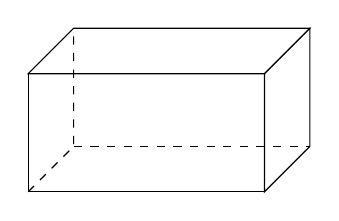
\begin{tikzpicture}
\pgfmathsetmacro{\cubex}{3}
\pgfmathsetmacro{\cubey}{1.5}
\pgfmathsetmacro{\cubez}{1.5}
\draw[black] (0,0,0) -- ++(-\cubex,0,0) -- ++(0,-\cubey,0) -- ++(\cubex,0,0) -- cycle;
\draw[black] (0,0,0) -- ++(0,0,-\cubez) -- ++(0,-\cubey,0) -- ++(0,0,\cubez) -- cycle;
\draw[black] (0,0,0) -- ++(-\cubex,0,0) -- ++(0,0,-\cubez) -- ++(\cubex,0,0) -- cycle;
\draw[black, dashed] (-\cubex, -\cubey, -\cubez) -- ++(\cubex, 0, 0);
\draw[black, dashed] (-\cubex, -\cubey, 0) -- ++(0,0,-\cubez) -- ++(0,\cubey,0);
\end{tikzpicture}
\end{figure}

Adding a single plane splits the cube into $2$ distinct spaces.
\begin{figure}[h!]
    \centering
    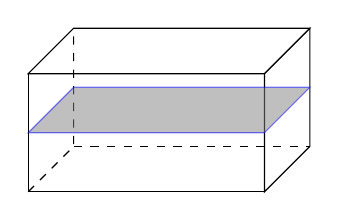
\begin{tikzpicture}
\pgfmathsetmacro{\cubex}{3}
\pgfmathsetmacro{\cubey}{1.5}
\pgfmathsetmacro{\cubez}{1.5}
\draw[black] (0,0,0) -- ++(-\cubex,0,0) -- ++(0,-\cubey,0) -- ++(\cubex,0,0) -- cycle;
\draw[black] (0,0,0) -- ++(0,0,-\cubez) -- ++(0,-\cubey,0) -- ++(0,0,\cubez) -- cycle;
\draw[black] (0,0,0) -- ++(-\cubex,0,0) -- ++(0,0,-\cubez) -- ++(\cubex,0,0) -- cycle;
\draw[black, dashed] (-\cubex, -\cubey, -\cubez) -- ++(\cubex, 0, 0);
\draw[black, dashed] (-\cubex, -\cubey, 0) -- ++(0,0,-\cubez) -- ++(0,\cubey,0);
\draw[blue,fill=gray,opacity=0.5] (-\cubex,-\cubey/2,0) -- ++(\cubex,0,0) -- ++(0,0,-\cubez) -- ++(-\cubex,0,0) -- cycle;
\end{tikzpicture}
\end{figure}

It is clear that we get $4$ separate spaces when there are $2$ planes. One may think it like this: the new vertical plane is divided into $2$ distinct regions by the previous horizontal plane. Their intersection is indicated by a solid line. For each of the divided region in the vertical plane, a single new space is introduced in addition to the previous one, thus we get $2 + 2 = 4$ total spaces.
\begin{figure}[h!]
    \centering
    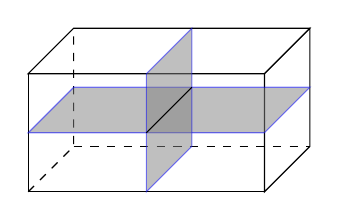
\begin{tikzpicture}
\pgfmathsetmacro{\cubex}{3}
\pgfmathsetmacro{\cubey}{1.5}
\pgfmathsetmacro{\cubez}{1.5}
\draw[black] (0,0,0) -- ++(-\cubex,0,0) -- ++(0,-\cubey,0) -- ++(\cubex,0,0) -- cycle;
\draw[black] (0,0,0) -- ++(0,0,-\cubez) -- ++(0,-\cubey,0) -- ++(0,0,\cubez) -- cycle;
\draw[black] (0,0,0) -- ++(-\cubex,0,0) -- ++(0,0,-\cubez) -- ++(\cubex,0,0) -- cycle;
\draw[black, dashed] (-\cubex, -\cubey, -\cubez) -- ++(\cubex, 0, 0);
\draw[black, dashed] (-\cubex, -\cubey, 0) -- ++(0,0,-\cubez) -- ++(0,\cubey,0);
\draw[blue,fill=gray,opacity=0.5] (-\cubex,-\cubey/2,0) -- ++(\cubex,0,0) -- ++(0,0,-\cubez) -- ++(-\cubex,0,0) -- cycle;
\draw[blue,fill=gray,opacity=0.5] (-\cubex/2,0,0) -- ++(0,-\cubey,0) -- ++(0,0,-\cubez) -- ++(0,\cubey,0) -- cycle;
\draw[black] (-\cubex/2, -\cubey/2, 0) -- ++(0,0,-\cubez);
\end{tikzpicture}
\end{figure}
\clearpage

Adding the $3$rd plane divides the cube into $8$ separate spaces. The $3$rd planes intersects with the previous $2$ planes, which gives $2$ intersection lines (indicated by the dotted black lines). These $2$ dotted lines divide the $3$rd plane into $4$ separate regions. For each of these regions, we get a new space in addition to the previous $4$, thus we get $4 + 4 = 8$ total spaces.
\begin{figure}[h!]
    \centering
    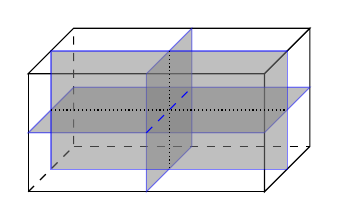
\begin{tikzpicture}
\pgfmathsetmacro{\cubex}{3}
\pgfmathsetmacro{\cubey}{1.5}
\pgfmathsetmacro{\cubez}{1.5}
\draw[black] (0,0,0) -- ++(-\cubex,0,0) -- ++(0,-\cubey,0) -- ++(\cubex,0,0) -- cycle;
\draw[black] (0,0,0) -- ++(0,0,-\cubez) -- ++(0,-\cubey,0) -- ++(0,0,\cubez) -- cycle;
\draw[black] (0,0,0) -- ++(-\cubex,0,0) -- ++(0,0,-\cubez) -- ++(\cubex,0,0) -- cycle;
\draw[black, dashed] (-\cubex, -\cubey, -\cubez) -- ++(\cubex, 0, 0);
\draw[black, dashed] (-\cubex, -\cubey, 0) -- ++(0,0,-\cubez) -- ++(0,\cubey,0);
\draw[blue,fill=gray,opacity=0.5] (-\cubex,-\cubey/2,0) -- ++(\cubex,0,0) -- ++(0,0,-\cubez) -- ++(-\cubex,0,0) -- cycle;
\draw[blue,fill=gray,opacity=0.5] (-\cubex/2,0,0) -- ++(0,-\cubey,0) -- ++(0,0,-\cubez) -- ++(0,\cubey,0) -- cycle;
\draw[blue,fill=gray,opacity=0.5] (-\cubex,0,-\cubez/2) -- ++(\cubex,0,0) -- ++(0,-\cubey,0) -- ++(-\cubex,0,0) -- cycle;
\draw[blue, dashed] (-\cubex/2, -\cubey/2, 0) -- ++(0,0,-\cubez);
\draw[black, densely dotted] (-\cubex/2, 0, -\cubez/2) -- ++(0,-\cubey,0);
\draw[black, densely dotted] (-\cubex, -\cubey/2, -\cubez/2) -- ++(\cubex,0,0);
\end{tikzpicture}
\end{figure}

\begin{figure}[h!]
    \centering
    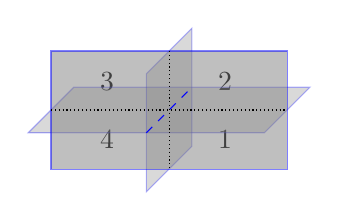
\begin{tikzpicture}
\pgfmathsetmacro{\cubex}{3}
\pgfmathsetmacro{\cubey}{1.5}
\pgfmathsetmacro{\cubez}{1.5}
\node at (-\cubex/6, -\cubey/1.8) {1};
\node at (-\cubex/6, -.1) {2};
\node at (-2, -.1) {3};
\node at (-2, -\cubey/1.8) {4};
\draw[blue,fill=gray,opacity=0.3] (-\cubex,-\cubey/2,0) -- ++(\cubex,0,0) -- ++(0,0,-\cubez) -- ++(-\cubex,0,0) -- cycle;
\draw[blue,fill=gray,opacity=0.3] (-\cubex/2,0,0) -- ++(0,-\cubey,0) -- ++(0,0,-\cubez) -- ++(0,\cubey,0) -- cycle;
\draw[blue,fill=gray,opacity=0.5] (-\cubex,0,-\cubez/2) -- ++(\cubex,0,0) -- ++(0,-\cubey,0) -- ++(-\cubex,0,0) -- cycle;
\draw[blue, dashed] (-\cubex/2, -\cubey/2, 0) -- ++(0,0,-\cubez);
\draw[black, densely dotted] (-\cubex/2, 0, -\cubez/2) -- ++(0,-\cubey,0);
\draw[black, densely dotted] (-\cubex, -\cubey/2, -\cubez/2) -- ++(\cubex,0,0);
\end{tikzpicture}
\end{figure}

We can see a pattern forming from the base cases. The $n$th plane is intersected by the previous $n-1$ planes, which can be though of as $n-1$ intersection lines through the $n$th plane. We know that the number of regions formed by $n-1$ lines through a plane is $L_{n-1}$. For each of these regions, we are getting a new space. So the number of new spaces is the same as $L_{n-1}$.\\

If we denote $P_n$ as the maximum number of $3$-dimensional spaces that can be defined by $n$ planes, we can define $P_n$ as:
\begin{align}
    P_n = P_{n-1} + L_{n-1}
\end{align}

\section*{Problem 15}
The problem is undefined for $n=1$, we will assume $n\geq2$. We can split the problem into two cases:
\begin{enumerate}[label=(\roman*)]
    \item Even number of people: If we start with $2n$ persons, after the first round all the even numbered persons will be eliminated. Just like the original problem, we can write:
          $$I(2n) = 2I(n) - 1$$
    \item Odd number of people: Similarly for this case, we can write:
          $$I(2n + 1) = 2I(n) + 1$$
\end{enumerate}
\begin{table}[h!]
    \centering
    \begin{tabular}{L|LLLLLLLLLLLL}
        n    & 1      & 2 & 3 & 4 & 5 & 6 & 7 & 8 & 9 & 10 & 11 & 12 \\ \hline
        I(n) & \times & 2 & 1 & 3 & 5 & 1 & 3 & 5 & 7 & 9  & 11 & 1
    \end{tabular}
    \caption*{First few values for the penultimate number}
    \label{tab:tab_15}
\end{table}
\clearpage
If we look at the values of $n$ for which $I(n) = 1$, we get $n = 3,6,12,\ldots = 3\times 2^0, 3\times2^1, 3\times2^2, \ldots$.

If we write $n = 3\times2^m + r$, where $m$ is the highest integer such that $3\times2^m\leq n$, then we can propose $I(n)= I(3\times2^m + r) = 2r + 1$. This formula checks out for other values as well, for example: $n=8=3\times2^2 + 2$, $I(8) = 2\times2 + 1 = 5$. This is our proposed hypothesis. We can use proof by induction to check if this is indeed correct.\\

\textit{Base case}: $n=2=3\times2^{-1} + \frac{1}{2} \implies I(\frac{1}{2})= 2\times \frac{1}{2} + 1 = 2$ \\

\textit{Inductive hypothesis:} Assume the formula holds for $m=2,3,\ldots,k$

$I(n)=I(3\times 2^k + r) = 2r+1$\\

\textit{Proof:} We have to show that the formula holds for $m=k+1$.

\begin{enumerate}[label=(\roman*)]
    \item $n = 3\times2^k + r$ even:
          \begin{align*}
                       & I(3\times 2^{(k+1)} + r)                                             \\
              \implies & I(3\times2^k\times2 + r)                                             \\
              \implies & 2I(3\times2^k + \frac{r}{2}) - 1 \qquad \text{Since $I(2n)=2I(n)-1$} \\
              \implies & 2(2\times\frac{r}{2} + 1) - 1                                        \\
              \implies & 2r + 1
          \end{align*}
    \item $n = 3\times2^k + r$ odd:
          \begin{align*}
                       & I(3\times 2^{(k+1)} + r)                                                 \\
              \implies & I(3\times2^k\times2 + (r-1)+1)                                           \\
              \implies & 2I(3\times2^k + \frac{r-1}{2}) + 1 \qquad \text{Since $I(2n+1)=2I(n)+1$} \\
              \implies & 2(2\times\frac{r-1}{2} + 1) + 1                                          \\
              \implies & 2r + 1
          \end{align*}
\end{enumerate}

Thus $I(n) = I(3\times2^m + r) = 2r + 1$ is the required formula for $n\geq2$.
\clearpage
\section*{Problem 17}
If we place the head of a zig inside another zig, we won't be able to achieve the maximum number of regions, $Z_n$. From the figure below, we can see that there are only $2$ intersection points and we have a total of $5$ regions.
\ctikzfig{fig17_1}

In order to maximize the number of regions, we would need to maximize the number of intersections as well. For that we have to place the head of each zigs outside the region of another one. In the figure below, we obtain $4$ intersection points and $7$ regions, which is the maximum possible number. The mapping from intersection points to the number of regions is distinct: We have $7$ regions if and only if we have $4$ intersection points. This holds for other values as well when the number of regions is maximized.
\ctikzfig{fig17_3}


Now let us think about a modified version of the problem. Suppose that each zigs has an angle of $90^{\circ}$. We know from the previous example that we can have at most $7$ regions with $2$ zigs, and those zigs must intersect at $4$ distinct points. When each of the two zigs is at $90^{\circ}$, no matter how hard we try, it is impossible to get more than $3$ intersection points, which gives a maximum of $6$ regions. There will always be at least one line for each zig that will keep diverging from another line of the other zig.
\begin{figure}[h!]
    \centering
    \tikzfig{fig17_2}
    \caption*{The dashed lines do not intersect and diverge from each other}
    \label{fig17_2}
\end{figure}

The reasoning is simple: two $90^{\circ}$s add up to $180^{\circ}$, in order to have $4$ intersection points, at least one of the zigs need to have an angle  $<90^{\circ}$. We can go the other way around: when the angle of each zigs is at $90^{\circ}$, we will have $< (\frac{180}{90} = 2)$ zigs that will give the maximum number of regions. For problem 17, the angle is $30^{\circ}$ and we will have $< (\frac{180}{30} = 6)$ zigs that can obtain $Z_n$ number of regions. The maximum integer $<6$ is $5$.
